\section{マイクロコンピュータ(青木)}
\noindent\large{\textbf{問1}}\quad 
  i=3,j=3,k=7の場合，次の式の結果を真(true)，偽(false)で答えなさい．\medskip\\
    \begin{tabular}{|
      >{\centering\arraybackslash}m{0.15\linewidth}|
      *{4}{>{\centering\arraybackslash}m{0.20\linewidth}|}
  }
      \hline
      \rule{0pt}{12pt} 式 & $i=j$ & $j!=k$ & $i<=j$ & $j>k$ \\ \hline
      \rule{0pt}{24pt} 式の結果 &  &  &  &  \\ \hline
    \end{tabular}
  \bigskip

\noindent\large{\textbf{問2}}\quad 
  x=5, y=10の場合，次の式の結果，xに代入される値を答えなさい．\medskip\\
    \begin{tabular}{|
        >{\centering\arraybackslash}m{0.15\linewidth}|
        *{3}{>{\centering\arraybackslash}m{0.20\linewidth}|}
    }
        \hline
        \rule{0pt}{12pt} 式 & $x=y++;$ & $x=y--;$ & $x+=10;$ \\ \hline
        \rule{0pt}{24pt} 式の結果 &  &  &  \\ \hline
    \end{tabular}
  \bigskip

\noindent\large{\textbf{問3}}\quad 
  次の文章の【】の中に適する言葉や関数を入れ，文章を完成させなさい．\\
  (a)【\ding{172}】制御は，LEDが点灯する明るさを変化させたい場合などに用いられ，\par
  ArduinoのD5ポートに接続したLEDをデューティ比80\%で【\ding{172}】制御により\par 
  点灯させるための関数は，【\ding{173}】となる．\\
  (b)1$\sim$1000の範囲の変数xに対し，Serial.println(100/1024*x)を実行するとxの\par
  値に関わらずシリアルモニタに表示されるのは0となる．0以外の計算結果を\par 
  表示するには，関数を【\ding{174}】に変更する．\medskip\\
  \renewcommand{\arraystretch}{1.5}
    \begin{tabular}{|m{0.33\linewidth}|m{0.66\linewidth}|}
    \hline
    \:\:\:\ding{172}&\:\:\:\ding{173} \\ \hline
    \multicolumn{2}{|m{\linewidth}|}{\ding{174}} \\ \hline
    \end{tabular}
  \bigskip

\noindent\large{\textbf{問4}}\quad 
  図(a)，(b)に示すマイコンの入力ピンに接続されたスイッチ入力回路に\par\quad ついて次の問いに答えなさい．\\
  (1)スイッチ(SW)のON，OFFに対して入力ピンに入力される電圧を答えな\par さい．
  \begin{figure}[H]
  \begin{minipage}{.4\textwidth}
    % \resizebox{0.45\linewidth}{!}{%
    \begin{tabular}{|
      >{\centering\arraybackslash}m{0.2\linewidth}|
      >{\centering\arraybackslash}m{0.38\linewidth}|
      >{\centering\arraybackslash}m{0.38\linewidth}|
    }
    \hline
    SW & 図(a)の入力電圧 & 図(b)の入力電圧 \\ \hline
    ON & & \\ \hline
    OFF & & \\ \hline
    \end{tabular}
    % }
  \end{minipage}
  \hfill
  \begin{minipage}{.4\textwidth}
    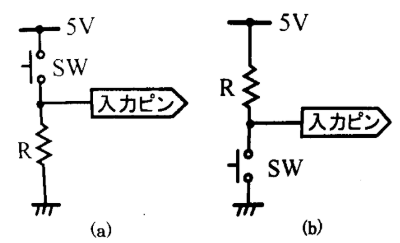
\includegraphics[width=\linewidth]{image/MicroCon1.png}
  \end{minipage}
  \end{figure}
  \medskip

  \noindent(2)プルアップと呼ばれる回路は(a)と(b)のどちらか答えなさい．
  \hfill
    \begin{tabular}{|c|}
    \hline
    答~~~~~~~~~~ \\
    \hline
    \end{tabular}
  \bigskip

  \begin{figure}[H]
  \begin{minipage}{.7\textwidth}
  \noindent\large{\textbf{問5}}\quad
  右図に示す5[V]の電源に接続されたLEDがある．\par\quad\quad
  点灯時のLEDの電圧降下(順方向電圧)が2.1[V]で，\par\quad\quad
  LEDに流す電流(順方向電流)が10[mA]とした場合\par\quad\quad
  の電流制限抵抗Rの値を求めなさい．\\
  \newline
  \hfill
    \begin{tabular}{|c|}
    \hline
    答~~~~~~~~~~~~~~~~~~~~ \\
    \hline
    \end{tabular}
  \end{minipage}
  \hfill
  \begin{minipage}{.2\textwidth}
    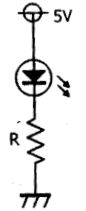
\includegraphics[width=0.55\linewidth]{image/MicroCon2.png}
  \end{minipage}
  \end{figure}
  \bigskip

\begin{figure}[H]
\begin{minipage}{.6\textwidth}
  \noindent\large{\textbf{問6}}\quad
  図1のようにArduinoのD8$\sim$D11ピンに\par\quad\quad
  LEDを接続した場合に，表1に示すように点\par\quad\quad
  灯した2個のLEDが1秒ごとに移動する\par\quad\quad
  プログラムを□を埋めて完成させなさい．\medskip\\
  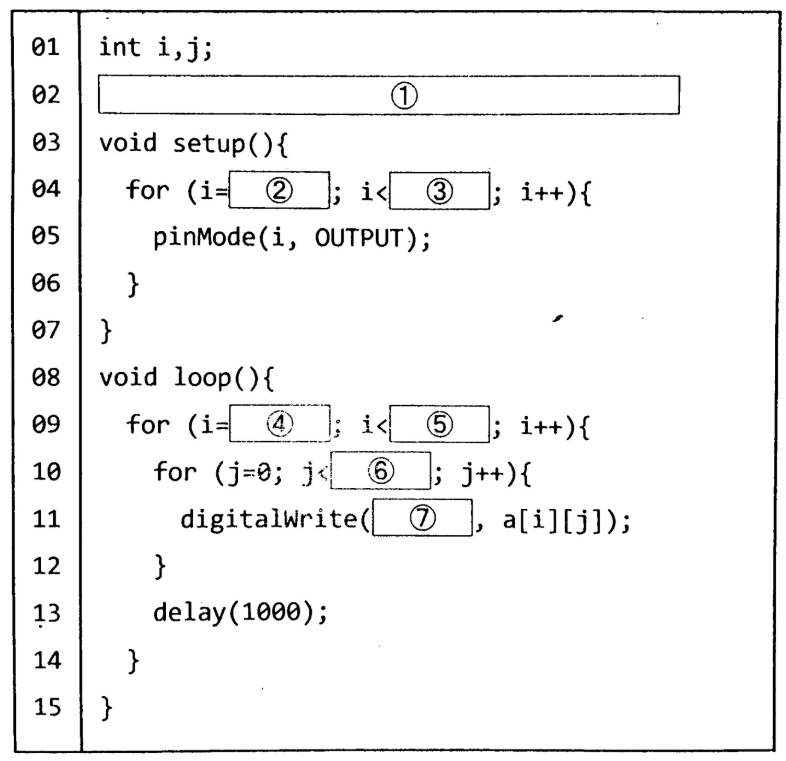
\includegraphics[width=0.95\linewidth]{image/MicroCon3.png}
\end{minipage}
\hfill
\begin{minipage}{.5\textwidth}
  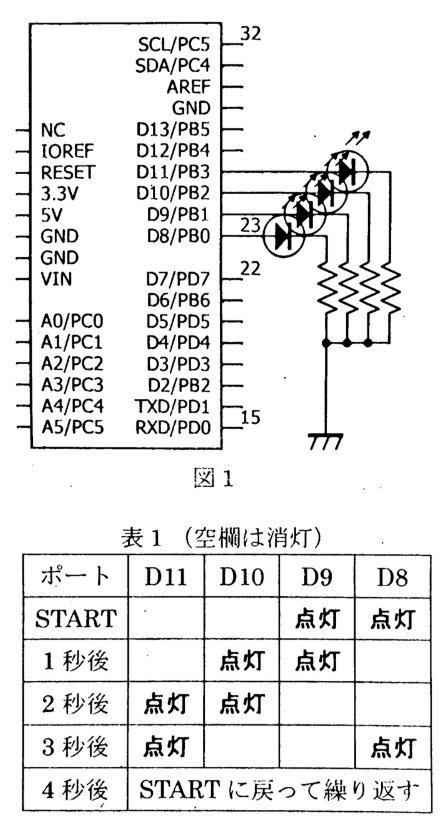
\includegraphics[width=0.85\linewidth]{image/MicroCon4.png}
\end{minipage}
\end{figure}

  \renewcommand{\arraystretch}{1.5}
    \begin{tabular}{|m{0.33\linewidth}|m{0.33\linewidth}|m{0.33\linewidth}|}
    \hline
    \multicolumn{3}{|m{\linewidth}|}{\ding{172}} \\ \hline
    \quad\:\:\:\ding{173}&\:\:\:\ding{174}&\:\:\:\ding{175} \\ \hline
    \quad\:\:\:\ding{176}&\:\:\:\ding{177}&\:\:\:\ding{178} \\ \hline
    \end{tabular}
  \bigskip

  \begin{figure}[H]
  \begin{minipage}{.7\textwidth}
  \noindent\large{\textbf{問7}}\quad
  右図のようにArduinoのD3ピンに接続された\par\quad\quad
  スイッチとD13ピンに接続されているオンボード\par\quad\quad
  LEDに対して，スイッチがOFFのときLEDが\par\quad\quad
  0.5秒周期で点滅(0.25秒間点灯，0.25秒間消灯)し，\par\quad\quad
  スイッチがONのときLEDが点灯するプログラム\par\quad\quad
  を作成しなさい．\\
  \end{minipage}
  \hfill
  \begin{minipage}{.2\textwidth}
    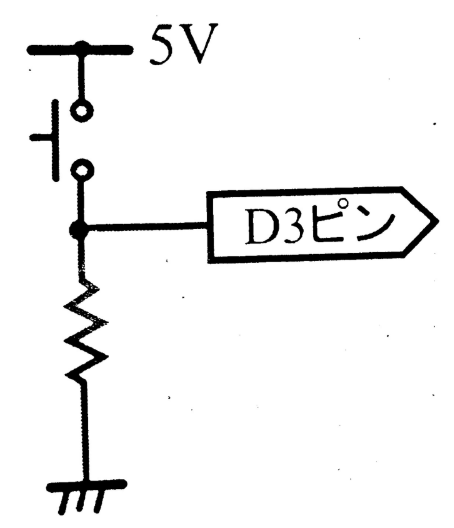
\includegraphics[width=1.4\linewidth]{image/MicroCon5.png}
  \end{minipage}
  \end{figure}
  \bigskip\bigskip\bigskip\bigskip\bigskip\bigskip
  \bigskip\bigskip\bigskip\bigskip\bigskip\bigskip
  \bigskip\bigskip\bigskip

\noindent\large{\textbf{問8}}\quad 
  図2のようにArduinoのD10ピンにLEDを接続し，D2$\sim$D3ピンにスイッ\par\quad チを接続した回路がある．
  □を埋めて以下の条件を満たすプログラムを完成\par\quad させなさい．
  なお，スイッチに抵抗が接続されていないことを考慮して，スイ\par\quad ッチの入力に対してプルアップ設定をしたプログラムを作成すること．\\
  【条件】
  \begin{itemize}
    \item 電源投入時，LEDは2秒周期で点滅する
    \item SW0が，ONのときLEDの点滅周期が100msずつ短くなり，OFFのとき点滅周期に変化はない
    \item SW1が，ONのときLEDの点滅周期が100msずつ長くなり，OFFのとき点滅周期に変化はない
    \item SW0とSW1が同時にONになることはない
    \item 点滅周期の最大値は10秒，最小値は100msとする
    \item 点滅周期は，1回の点灯時間と消灯時間をあわせた時間とする
  \end{itemize}

  \begin{figure}[H]
  \begin{minipage}{.6\textwidth}
    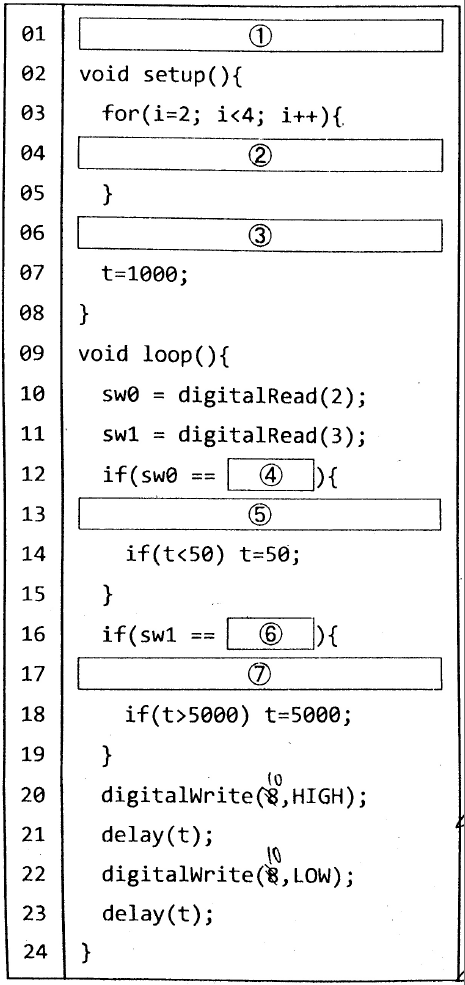
\includegraphics[width=0.8\linewidth]{image/MicroCon6.png}
  \end{minipage}
  \hfill
  \begin{minipage}{.4\textwidth}
    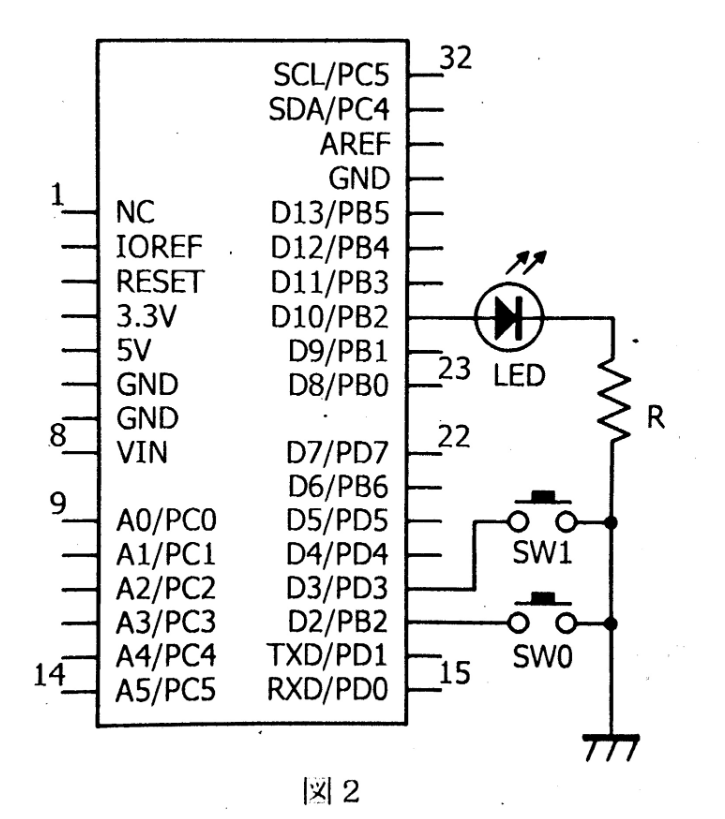
\includegraphics[width=1.1\linewidth]{image/MicroCon7.png}
    \medskip
    \renewcommand{\arraystretch}{2}
      \begin{tabular}{|m{0.33\linewidth}|m{0.33\linewidth}|m{0.33\linewidth}|}
      \hline
      \multicolumn{3}{|m{\linewidth}|}{\ding{172}} \\ \hline
      \multicolumn{3}{|m{\linewidth}|}{\ding{173}} \\ \hline
      \multicolumn{3}{|m{\linewidth}|}{\ding{174}} \\ \hline
      \multicolumn{3}{|m{\linewidth}|}{\ding{175}} \\ \hline
      \multicolumn{3}{|m{\linewidth}|}{\ding{176}} \\ \hline
      \multicolumn{3}{|m{\linewidth}|}{\ding{177}} \\ \hline
      \end{tabular}
  \end{minipage}
  \end{figure}
  \bigskip
  \newpage

\noindent\large{\textbf{問9}}\quad 
以下に示すプログラムがそれぞれ実行された場合，シリアルモニタに表示\par\quad される文字列を答えなさい．
\begin{center}  
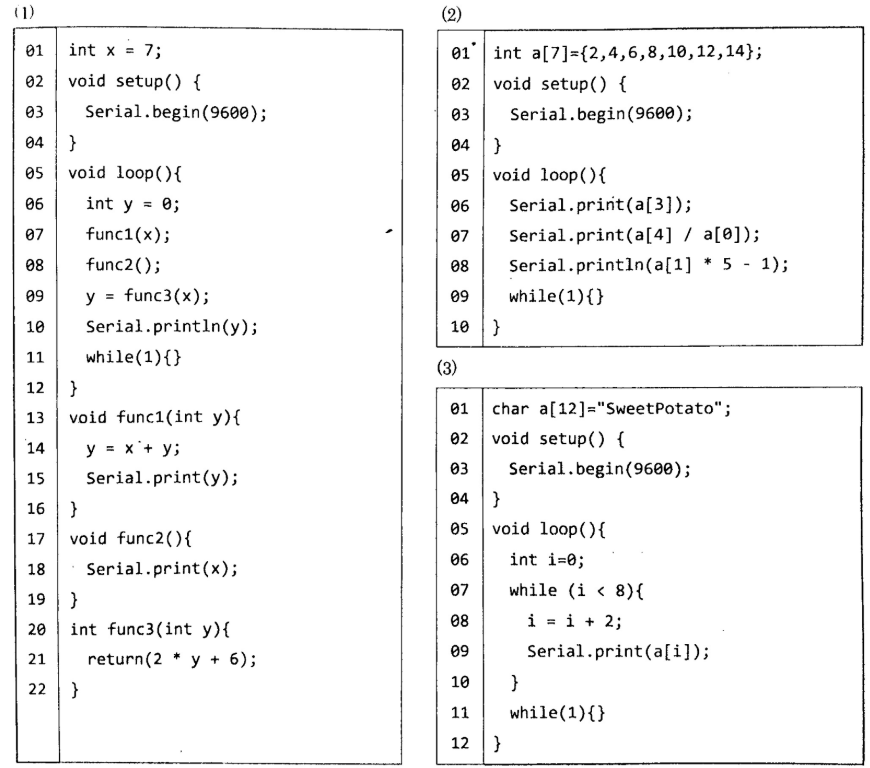
\includegraphics[width=0.9\linewidth]{image/MicroCon8.png}
\end{center}
  \begin{tabular}{|m{0.5\linewidth}|m{0.5\linewidth}|}
    \hline
    \:\:\:(1)&\:\:\:(2) \\ \hline
    \:\:\:(3)&\\ \hline
  \end{tabular}
  \bigskip

\begin{center}
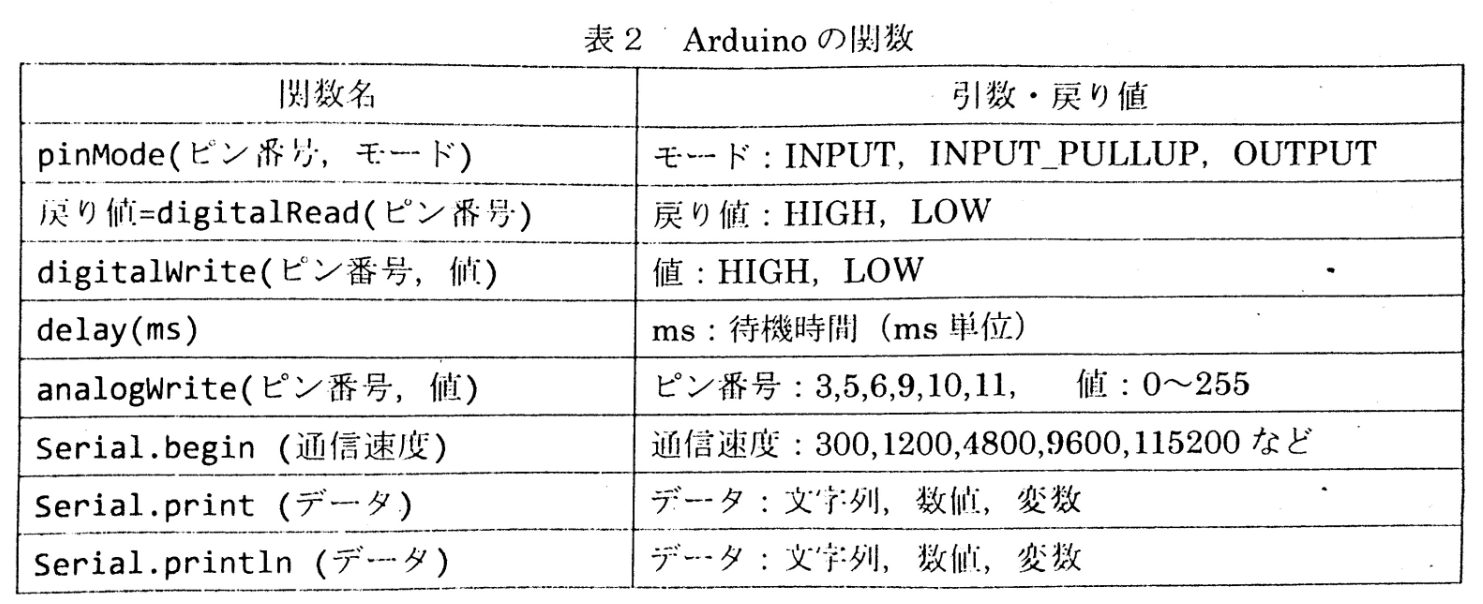
\includegraphics[width=0.88\linewidth]{image/MicroCon9.png}
\end{center}